\documentclass[10pt,twoside]{pnas-new}
% Use the lineno option to display guide line numbers if required.

\templatetype{pnasmathematics} % Choose template 
% {pnasresearcharticle} = Template for a two-column research article
% {pnasmathematics} = Template for a one-column mathematics article
% {pnasinvited} = Template for a PNAS invited submission

%remove watermark
\setboolean{displaywatermark}{false}

\title{Topological  Fractal  Dimension  of  Networks  of Protein–Protein  Interaction  Networks}
%PNAS LaTeX Template for preparing single-column mathematics articles on Overleaf
% Use letters for affiliations, numbers to show equal authorship (if applicable) and to indicate the corresponding author
\author[a]{Georgios Kalantzis}
\author[a]{Andrei Stoica} 

\affil[a]{SABS, DTC}

% Please give the surname of the lead author for the running footer
%\leadauthor{Lead author last name} 

% Please add here a significance statement to explain the relevance of your work
\significancestatement{Authors must submit a 120-word maximum statement about the significance of their research paper written at a level understandable to an undergraduate educated scientist outside their field of speciality. The primary goal of the Significance Statement is to explain the relevance of the work in broad context to a broad readership. The Significance Statement appears in the paper itself and is required for all research papers.}

% Please include corresponding author, author contribution and author declaration information
%\authorcontributions{Please provide details of author contributions here.}
%\authordeclaration{Please declare any conflict of interest here.}
%\equalauthors{\textsuperscript{1}A.O.(Author One) and A.T. (Author Two) contributed equally to this work (remove if not applicable).}
%\correspondingauthor{\textsuperscript{2}To whom correspondence should be addressed. E-mail: author.two\@email.com}

% Keywords are not mandatory, but authors are strongly encouraged to provide them. If provided, please include two to five keywords, separated by the pipe symbol, e.g:
\keywords{PPIN $|$ NetworkX $|$ BioGrid $|$ Network Science $|$ Centrality Measures} 

\begin{abstract}
Please provide an abstract of no more than 250 words in a single paragraph. Abstracts should explain to the general reader the major contributions of the article. References in the abstract must be cited in full within the abstract itself and cited in the text.
\end{abstract}

\dates{This manuscript was compiled on \today}
%\doi{\url{www.pnas.org/cgi/doi/10.1073/pnas.XXXXXXXXXX}}

\begin{document}

\maketitle
\thispagestyle{firststyle}
\ifthenelse{\boolean{shortarticle}}{\ifthenelse{\boolean{singlecolumn}}{\abscontentformatted}{\abscontent}}{}

\section{Introduction \& Prerequisites}
Networks are representations of real systems where individual units are modelled as nodes and interactions between these units as links. Formally speaking, this corresponds to a graph $\mathcal{G} = (\mathcal{V},\mathcal{E})$, with $\mathcal{V}$ and $\mathcal{E}$ standing for the set of nodes and edges respectively. However, nodes can be anything, ranging from regions of the human brain to electrical power plants. As a result, the study of networks pervades all of science, from neurobiology to statistical physics~\cite{strogatz2001exploring}.  

The set of nodes $\mathcal{V}$ has usually a finite number of elements. Links can be undirected or directed, unweighted or weighted. When dealing with undirected edges, a link can be defined as a pair of nodes $(u,v)$; in directed graphs $(u,v)$ and $(v,u)$ correspond to different edges. In the case of weighted networks, links are also assigned with a real number characterising the importance of the association.

There are two main ways for representing networks, namely lists and adjacency matrices. Let $\mathbf{A}$ be the adjacency matrix of graph  $\mathcal{G}$ containing $n$ nodes. Then $\mathbf{A}$ is of size $n\times n$ and element $A_{ij}$ is $1$ if nodes $i,j$ are connected, otherwise, $A_{ij}=0$. In weighted networks non-zero elements of $\mathbf{A}$ are equal to the weights of edges. Moreover, real complex networks, although might contain thousands of nodes, are usually sparse in regards of edges and can be represented by sparse matrices which are special data structures.

After defining nodes and edges, the next important term is that of node-degree. The degree $k_i$ of node $i$ is defined as the number of edges linked to $i$. In directed graphs, the degree of a node might be discriminated in in-degree and out-degree, depending on whether the edges ending to or start from $i$ are counted. For undirected networks, the degree can be computed by
\[ k_i = \sum_{j=1}^{n}A_{ij} = \mathbf{e}_i^\top ( \mathbf{A} \cdot \mathbf{e} ), \]
where  $\mathbf{e}$ stands for a column-vector full of ones and $\mathbf{e}_i$ has zeros everywhere except element $i$ which is one. In other words, the product $ \mathbf{A} \cdot \mathbf{e} $ gives the degree for every node. These are some simple indicators showing why adjacency matrices are important: they connect Network Science with Linear Algebra.

Graphs are very attractive tools to biological and medical research applications, since they can use for description of many mechanisms or interactions, for instance metabolic or cell signalling networks. Another important direction are the so-called Protein-Protein Interaction Networks (which will be denoted as PPIN), which represent physical contacts between proteins within a cell. In brief, 
proteins are macromolecules, consisting of one or more long chains of amino acid residues, which perform a vast array of functions within organisms, including catalysing metabolic reactions, DNA replication, responding to stimuli, providing structure to cells and organisms, and transporting molecules from one location to another. Usually, the aforementioned procedures incorporate the cascade of many proteins, resulting in networks of interactions.

PPINs are characterised by three notable properties. First of all, PPINs show a small world effect meaning that there is great connectivity between proteins. More typically, the diameter (the maximum number of steps separating any two nodes) of such networks is small, regardless the number of nodes or edges. Such strong connectivity has important biological consequences, since it allows for an efficient and quick flow of signals within the network~\cite{PPINtrain}.

Moreover, PPINs are scale-free. This class of networks can describe a variety of complex systems where some nodes have a tremendous number edges (hubs), whereas most nodes have only a few~\cite{barabasi2003scale}. In this sense, the network appears to have no scale which provides important features. For instance, scale-free networks are very robust and stable since small perturbations have low effect. Furthermore, hubs in cancer-linked networks could be used for targeted attacks in drug discovery.

Finally, another crucial characteristic of PPINs is their modularity. The transitivity or clustering coefficient of a network is a measure of the tendency of the nodes to cluster together. High transitivity means that the network contains communities or groups of nodes that are densely connected internally. Generally speaking, structure always affects function~\cite{strogatz2001exploring}. In biological networks particularly, finding these communities is very important, because they can reflect functional modules and protein complexes.

However, PPINs are not real but correspond to actual biological networks and occur after experimental procedures. As a result, data might contain noise and some observations can be less reliable since the record of molecular interactions is occasionally incomplete or patchy.

\section{Construction of PPIN and Analysis}
\label{sec:2-task1}
There are various software packages or programmatic methods available to build and analyse networks. Throughout this project we work mainly with \textsc{Python} and the \textsc{NetworkX} module. Furthermore, there are a lot of sources from which you can obtain and integrate PPI data, other than creating new experimental results. Current databases are distinguished in primary or predicting, depending on whether they just provide evidence or combine other resources for prediction. For the aims of this project we will be working with data from \textsc{BioGrid}, which is a primary curated biological database of protein-protein interactions, genetic interactions, chemical interactions, and post-translational modifications.

\subsection{Hands-on \textsc{BioGrid} \& \textsc{NetworkX}}

PPINs can be created from edge-lists, which are text files containing rows of the form ``$\text{ID}_A - \text{ID}_B$''. The latter correspond to distinctive labels of nodes which can also be used as reference  to other information sources. After loading an edge-file, \textsc{NetworkX} can initialise a graph with the provided edges.

\subsection{Analysis \& Illustration of PPIN}
Report/PNAS-template-main.tex

\subsection{Centrality \& Important Proteins}
By using PageRank, HITS and Degree Centrality we find that the five most ``central'' nodes are

\begin{table}[h]%[tbhp]
	\centering
	\caption{Top-5 Central Proteins in \textit{Homo Sapiens}}
	\begin{tabular}{cccl}
		Node Label & Protein & Gene & Function \\
		\midrule
		114030 & Cullin-3 & CUL3 & This protein plays a critical role in the polyubiquitination and subsequent degradation of specific protein substrates \\
		113164 & HMG20 &  UBC & It plays a key role in maintaining cellular ubiquitin levels under stress. Defects could lead to embryonic lethality. \\
		108309 & HuR & ELAVL1 & RNA-binding protein that binds to the 3'-UTR region of mRNAs and increases their stability \\
		113348 & Exportin-1 & XPO1 &  eukaryotic protein that mediates the nuclear export of proteins, rRNA, snRNA, and some mRNA. \\
		113010 & TP53 & TP53 & tumor suppressor protein containing transcriptional activation, DNA binding, and oligomerization domains.  \\
		\bottomrule
		\label{tab:central}
	\end{tabular}
\end{table}

%\[ 114030,\ 113164,\ 108309,\ 113348,\ 113010. \]
\subsection{Opt: Computational Complexity}

\subsection{Opt: The Development of PPINs} 


\section{Computing the Topological Fractal Dimension}
\label{sec:3-task2}
\subsection{The Box Counting Method}

\subsection{Implementation}

\subsection{Computational Complexity}

\section{TFD of PPIN \& Conclusions}
\label{sec:4-task3}
\begin{wraptable}{r}{9cm}
%\begin{table}[h!] %[tbhp]
\def\rownumber{} % hack for re-starting row-counter (and skip the header) 
	%\centering
    \caption{TFD calculation of PPINs on full graph or LCC }
    \label{table:tfd}
    \begin{tabular}{ @{ \makebox[2em][r]{\rownumber\space} } | lcc}
    	
		\textbf{Organism} & \textbf{TFD-full} &  \textbf{TFD-LCC} 
        \gdef\rownumber{\stepcounter{magicrownumbers} \arabic{magicrownumbers} } \\
		\midrule
        %$ Anopheles \ gambiae \ PEST $ & 1.0 & 1.0 \\ 
        $ Anopheles \ gambiae \ PEST $ & 1.0 & 1.0 \\ 
        %$ Apis \ mellifera $ & 1.0 & 1.0 \\ 
        $ Arabidopsis \ thaliana \ Columbia $ & 1.936 & 3.68 \\ 
        %$ Bacillus \ subtilis \ 168 $ & 0.585 & 1.0 \\ 
        %$ Bos \ taurus $ & 0.61 & 1.465 \\ 
        %$ Caenorhabditis \ elegans $ & 1.634 & 3.285 \\ 
        %$ Candida \ albicans \ SC5314 $ & 1.176 & 2.649 \\ 
        %$ Canis \ familiaris $ & 0.591 & 1.104 \\ 
        %$ Cavia \ porcellus $ & 0.75 & 0.585 \\ 
        %$ Chlamydomonas \ reinhardtii $ & 1.302 & 2.032 \\ 
        %$ Chlorocebus \ sabaeus $ & 0.892 & 0.955 \\ 
        %$ Cricetulus \ griseus $ & 1.082 & 2.084 \\ 
        %$ Danio \ rerio $ & 0.918 & 2.354 \\ 
        $ Dictyostelium \ discoideum \ AX4 $ & 1.171 & 1.342 \\ 
        %$ Drosophila \ melanogaster $ & 2.66 & 3.838 \\ 
        %$ Emericella \ nidulans \ FGSC \ A4 $ & 1.696 & 2.875 \\ 
        %$ Equus \ caballus $ & 1.0 & 1.0 \\ 
        %$ Escherichia \ coli \ K12 $ & 1.0 & 1.0 \\ 
        %$ Escherichia \ coli \ K12 \ MC4100 \ BW2952 $ & 0.796 & 1.001 \\ 
        %$ Escherichia \ coli \ K12 \ MG1655 $ & 1.303 & 3.31 \\ 
        $ Escherichia \ coli \ K12 \ W3110 $ & 4.913 & 4.913 \\ 
        %$ Gallus \ gallus $ & 1.058 & 2.511 \\ 
        %$ Glycine \ max $ & 1.438 & 2.155 \\ 
        $ Hepatitus \ C \ Virus $ & 3.399 & 3.948 \\ 
        $ Homo \ sapiens $ & 3.469 & 4.725 \\ 
        $ Human \ Herpesvirus \ 1 $ & 2.466 & 2.466 \\ 
        %$ Human \ Herpesvirus \ 2 $ & 0.775 & 0.955 \\ 
        %$ Human \ Herpesvirus \ 3 $ & 1.0 & 1.0 \\ 
        %$ Human \ Herpesvirus \ 4 $ & 1.828 & 2.732 \\ 
        %$ Human \ Herpesvirus \ 5 $ & 1.445 & 2.334 \\ 
        %$ Human \ Herpesvirus \ 6A $ & 0.892 & 1.171 \\ 
        $ Human \ Herpesvirus \ 6B $ & 0.775 & 0.585 \\ 
        %$ Human \ Herpesvirus \ 7 $ & 1.0 & 1.0 \\ 
        %$ Human \ Herpesvirus \ 8 $ & 1.107 & 2.356 \\ 
        $ Human \ Immunodeficiency \ Virus \ 1 $ & 4.395 & 4.395 \\ 
        %$ Human \ Immunodeficiency \ Virus \ 2 $ & 0.908 & 1.281 \\ 
        %$ Human \ papillomavirus \ 16 $ & 1.289 & 1.605 \\ 
        %$ Macaca \ mulatta $ & 1.342 & 1.962 \\ 
        %$ Meleagris \ gallopavo $ & 1.0 & 1.0 \\ 
        %$ Mus \ musculus $ & 2.008 & 3.803 \\ 
        %$ Mycobacterium \ tuberculosis \ H37Rv $ & 1.416 & 1.803 \\ 
        %$ Neurospora \ crassa \ OR74A $ & 1.484 & 1.71 \\ 
        %$ Nicotiana \ tomentosiformis $ & 1.0 & 1.0 \\ 
        %$ Oryctolagus \ cuniculus $ & 1.011 & 2.265 \\ 
        %$ Oryza \ sativa \ Japonica $ & 1.088 & 2.102 \\ 
        %$ Ovis \ aries $ & 1.0 & 1.0 \\ 
        %$ Pan \ troglodytes $ & 1.0 & 1.0 \\ 
        %$ Pediculus \ humanus $ & 1.0 & 1.0 \\ 
        %$ Plasmodium \ falciparum \ 3D7 $ & 1.833 & 2.939 \\ 
        %$ Rattus \ norvegicus $ & 1.383 & 2.956 \\ 
        % $ Ricinus \ communis $ & 0.955 & 0.955 \\ 
         $ Saccharomyces \ cerevisiae \ S288c $ & 4.822 & 4.822 \\ 
        % $ Schizosaccharomyces \ pombe \ 972h $ & 2.558 & 3.882 \\ 
        % $ Selaginella \ moellendorffii $ & 1.518 & 1.518 \\ 
        % $ Simian \ Immunodeficiency \ Virus $ & 1.196 & 1.171 \\ 
        % $ Simian \ Virus \ 40 $ & 1.484 & 1.484 \\ 
        % $ Solanum \ lycopersicum $ & 1.222 & 1.617 \\ 
        % $ Solanum \ tuberosum $ & 0.737 & 0.0 \\ 
        % $ Strongylocentrotus \ purpuratus $ & 2.311 & 2.311 \\ 
        % $ Sus \ scrofa $ & 0.86 & 1.854 \\ 
        % $ Tobacco \ Mosaic \ Virus $ & 0.955 & 0.955 \\ 
        % $ Ustilago \ maydis \ 521 $ & 1.171 & 1.171 \\ 
        % $ Vaccinia \ Virus $ & 0.87 & 0.955 \\ 
        % $ Vitis \ vinifera $ & 1.0 & 1.0 \\ 
        % $ Xenopus \ laevis $ & 1.073 & 2.56 \\ 
        % $ Zea \ mays $ & 0.703 & 0.585 \\ 
                %[1ex] 
		\bottomrule
	\end{tabular}	
%\end{table}
\end{wraptable}
We are now ready to comment on the final part of our project, which is the TFD calculation for various PPINs. After implementing the box covering algorithm, we tested it in two versions of PPINs for each of the $66$ organisms, on the complete graph with isolated nodes or disconnected components, as well as on the largest connected component (LCC). The results could be grouped in the following three cases. Firstly, the fully connected networks which showed no difference, those which had disconnected components but TFD was on similar values and, thirdly, some organism which resulted in significantly different TFD between the whole graph and the largest connected component. 

Table~\ref{table:tfd} summarizes the TFD of several PPIN, for both scenarios. $Anopheles gambiae PEST$ is an organism, among other, whose trivial PPIN -- two nodes with one edge -- is depicted in a TFD of $1$. \textit{HIV-1}, as stated earlier, has a fully connected PPIN and this is in accordance with the equality of the two TFDs.  



\begin{figure}[h]
	\begin{minipage}{0.45\textwidth}
    	\centering
		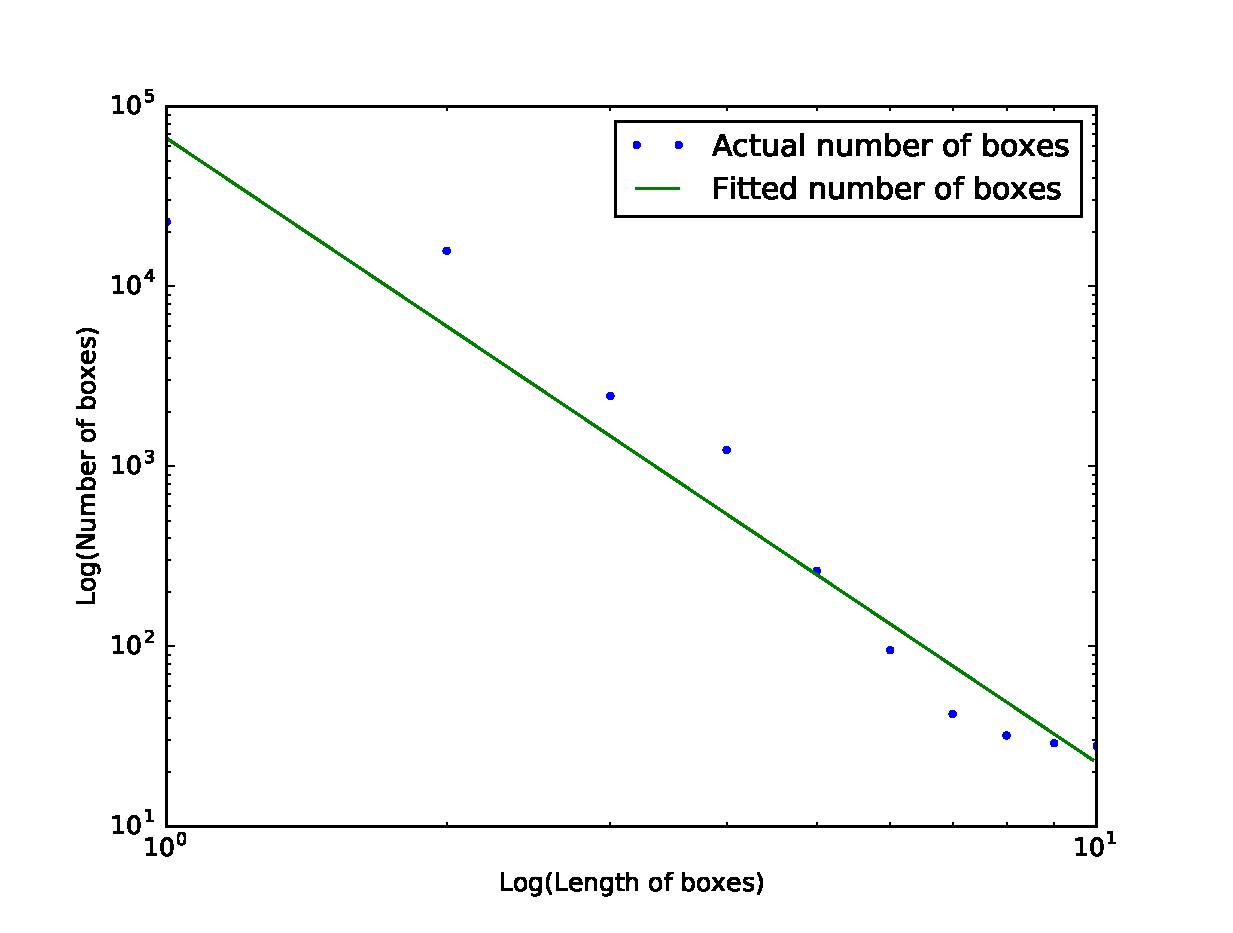
\includegraphics[width=\textwidth]{Graphics/Homo_sapiens_WG.eps}
        \caption{Data fitting on \textit{Homo sapiens} complete PPIN}
        \label{fig:HSWG}
	\end{minipage}
	%\hfill
	\begin{minipage}{0.45\textwidth}
		\centering
		%\vspace{10pt} % Hack for correct positioning
		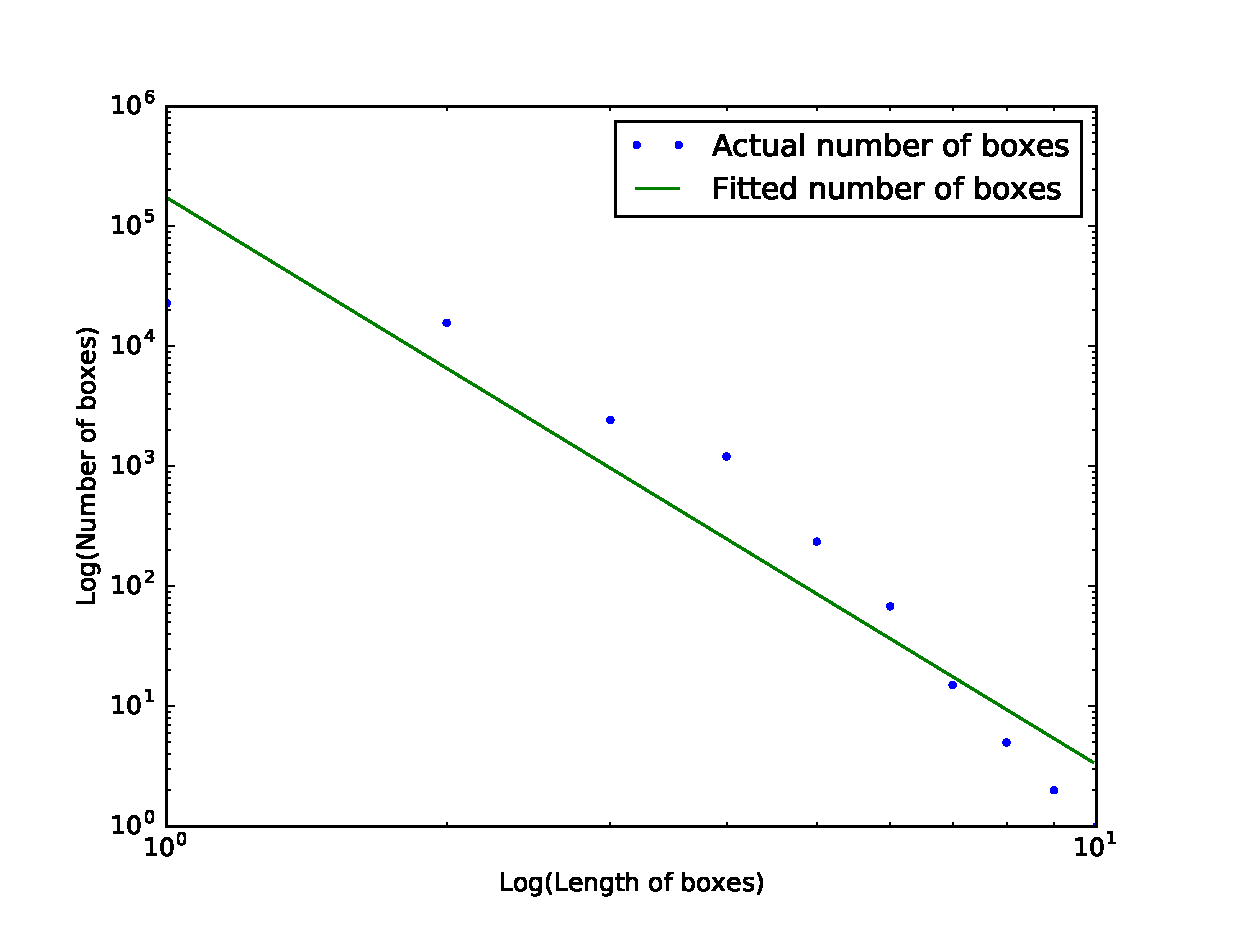
\includegraphics[width=\textwidth]{Graphics/Homo_sapiens_LCC.eps}
        \caption{Data fitting on the largest connected component of Homo sapiens PPIN}
		\label{fig:HSLCC}
	\end{minipage}
\end{figure}

The diagrams of Figures~\ref{fig:HSWG}-\ref{fig:HSLCC} present the number of boxes required for graph covering as a function of the box-side length, in a logarithmic scale. The estimated pairs are depicted as blue dots whereas green lines correspond to the linear-fit approximation.    

\subsection*{Code and Scripts} For the sake of efficiency and productivity we used a \textsc{GitHub} repository \footnote{ \url{github.com/giorkala/Protein-Protein-Interaction-Networks-Project/tree/master/PPIN_Construction}} with all our scripts and functions. After providing the initial dataset, it should work as a pipeline following the directions in comments or descriptions.

%\subsection*{Conclusions}


\subsection{Dynamic changes of TFD \& Interaction with other Databases}

\subsection{Conclusions}



\subsection*{Manuscript Length}

The maximum length of a Direct Submission research article is six pages and a Direct Submission Plus research article is ten pages including all text, spaces, and the number of characters displaced by figures, tables, and equations.  When submitting tables, figures, and/or equations in addition to text, keep the text for your manuscript under 39,000 characters (including spaces) for Direct Submissions and 72,000 characters (including spaces) for Direct Submission Plus.


\subsection*{Data Archival}

PNAS must be able to archive the data essential to a published article. Where such archiving is not possible, deposition of data in public databases, such as GenBank, ArrayExpress, Protein Data Bank, Unidata, and others outlined in the Information for Authors, is acceptable.

\subsection*{Language-Editing Services}
Prior to submission, authors who believe their manuscripts would benefit from professional editing are encouraged to use a language-editing service (see list at www.pnas.org/site/authors/language-editing.xhtml). PNAS does not take responsibility for or endorse these services, and their use has no bearing on acceptance of a manuscript for publication. 

%\begin{figure}%[tbhp]
%\centering
%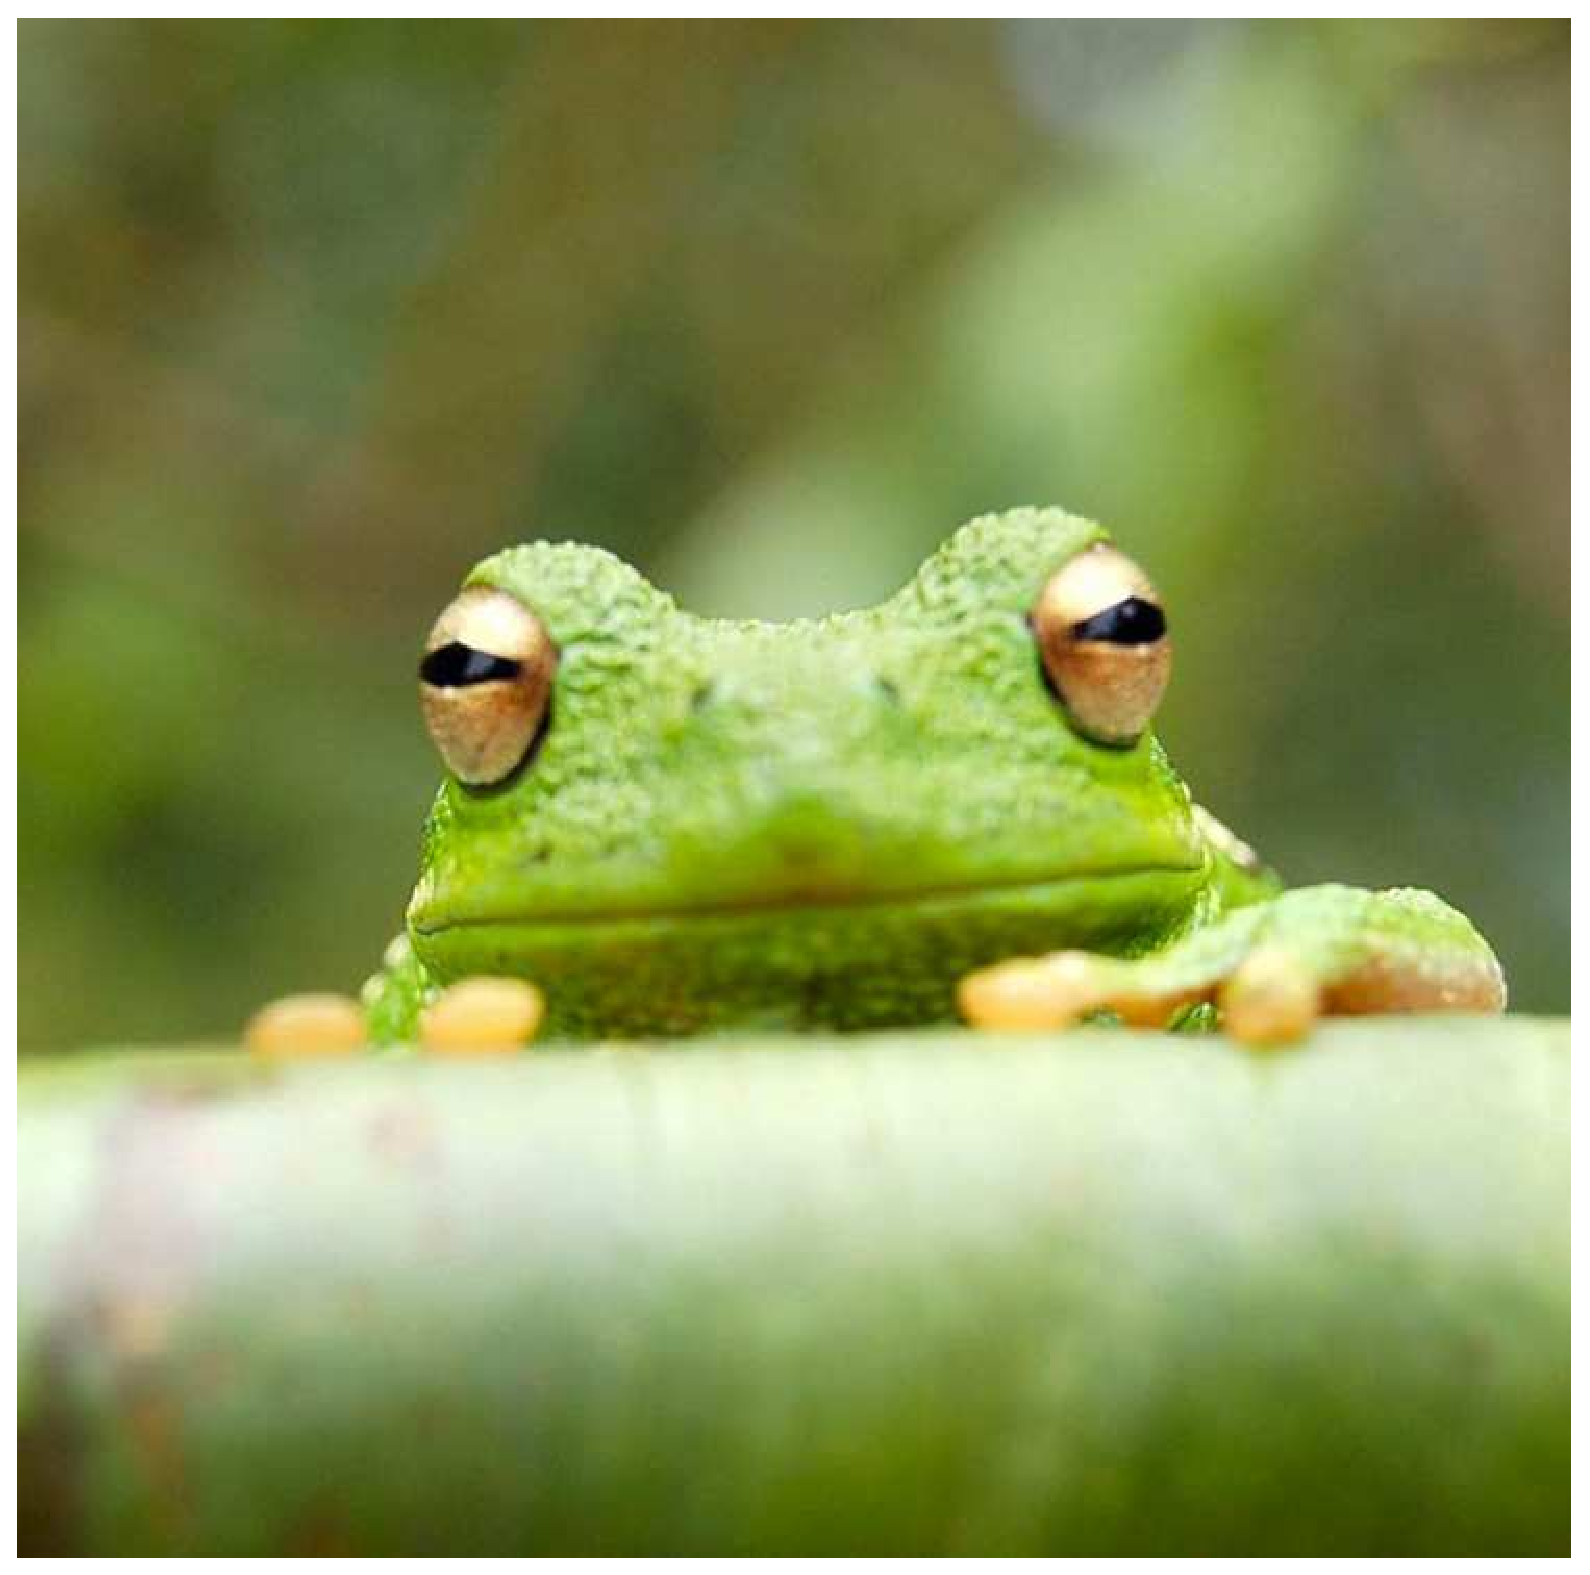
\includegraphics[width=.5\linewidth]{frog}
%\caption{Placeholder image of a frog with an example caption.}
%\label{fig:frog}
%\end{figure}


%\begin{SCfigure*}[\sidecaptionrelwidth][t]
%\centering
%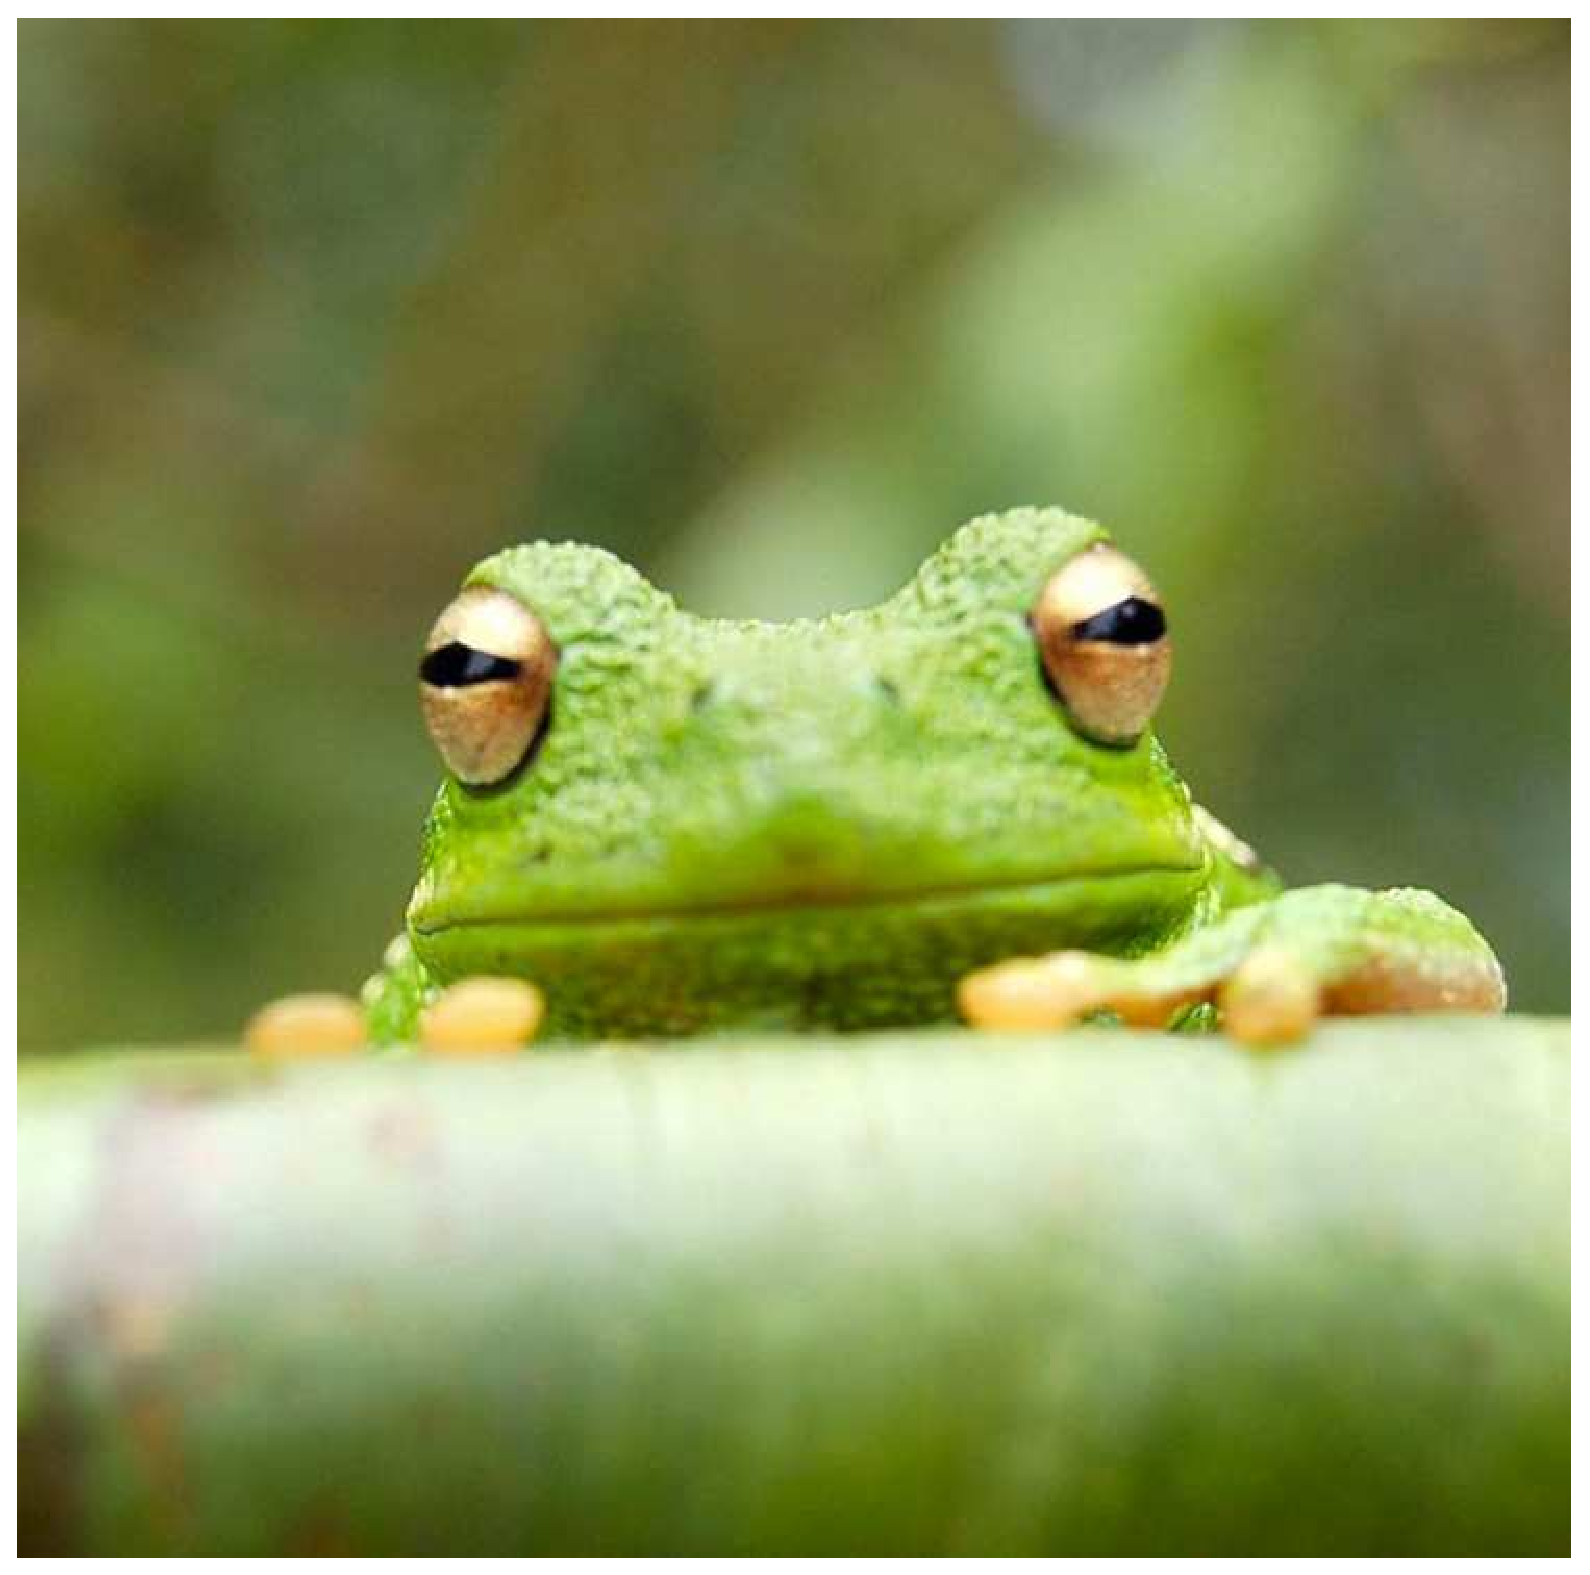
\includegraphics[width=11.4cm,height=11.4cm]{frog}
%\caption{This caption would be placed at the side of the figure, rather than below it.}\label{fig:side}
%\end{SCfigure*}


%\subsection*{Digital Figures}
%Only TIFF, EPS, and high-resolution PDF for Mac or PC are allowed for figures that will appear in the main text, and images must be final size. Authors may submit U3D or PRC files for 3D images; these must be accompanied by 2D representations in TIFF, EPS, or high-resolution PDF format.  Color images must be in RGB (red, green, blue) mode. Include the font files for any text. 

\subsection*{Supporting Information (SI)}

Authors should submit SI as a single separate PDF file, combining all text, figures, tables, movie legends, and SI references.  PNAS will publish SI uncomposed, as the authors have provided it.  Additional details can be found here: \href{http://www.pnas.org/page/authors/journal-policies}{policy on SI}.  For SI formatting instructions click \href{https://www.pnascentral.org/cgi-bin/main.plex?form_type=display_auth_si_instructions}{here}.  The PNAS Overleaf SI template can be found \href{https://www.overleaf.com/latex/templates/pnas-template-for-supplementary-information/wqfsfqwyjtsd}{here}.  Refer to the SI Appendix in the manuscript at an appropriate point in the text. Number supporting figures and tables starting with S1, S2, etc.

Authors who place detailed materials and methods in an SI Appendix must provide sufficient detail in the main text methods to enable a reader to follow the logic of the procedures and results and also must reference the SI methods. If a paper is fundamentally a study of a new method or technique, then the methods must be described completely in the main text.



\acknow{Please include your acknowledgments here, set in a single paragraph. Please do not include any acknowledgments in the Supporting Information, or anywhere else in the manuscript.}

\showacknow % Display the acknowledgements section
% Bibliography
\bibliography{PPIN-TFD_Literature}

\end{document}
